\scanpage{401}
\mspage{203}

\unsure{arithmétisations|arithmétisation} de $\pi'_i$ --- ce qui
reviendrait à la bijectivité de
\[
\widehat{\widehat{\mathcal T}}/\mathcal N_a
\longrightarrow
\widehat{\widehat{\mathcal G}}'/\unsure{M_{a'}^{\natural}|M_{a'}^{\sharp}}
\simeq \widehat{\widehat{\mathcal T}}'/\mathcal N_{a'},
\]
qui n'a\inserted{urait} guère de raison d'être que si
on admettait
$\widehat{\widehat{\mathcal T}}(\pi)\xrightarrow{\sim}\unsure{\widehat{\widehat{\mathcal G}}|\widehat{\mathcal G}}(\pi'_i)$,
qui me semble bien problématique.

\margin{\figure{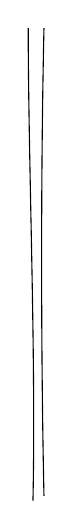
\begin{tikzpicture}[x=1cm,y=1cm,baseline=(current bounding box.north)]
\draw[line width=0.4pt] (0,0) .. controls (0.04,1.85) and (-0.06,4.30) .. (-0.06,6.00);
\draw[line width=0.4pt] (0.14,0.06) .. controls (0.10,1.90) and (0.10,4.25) .. (0.14,6.00);
\end{tikzpicture}}}
Cependant, on trouve, par le foncteur
"bouchage des trous", une équivalence
entre la catégorie des \deleted{\unsure{courbes alg.}}
groupes profinis à lacets \uuline{extérieurs} \uline{arithmétisés},
\inserted{de type $(g,\nu)$,}
et des groupes profinis à lacets
(pas extérieurs !) \uline{arithmétisés}, de type
$(g,\nu-1)$.

On peut se proposer d'essayer de
préciser \deleted{\unsure{par}} le type des propriétés
qui vont caractériser $\mathcal N_{g,\nu}$ dans $\mathcal N'_{g,\nu}=$
$\operatorname{Norm}_{\widehat{\widehat{\mathcal T}}_{g,\nu}}
(\widehat{\mathcal T}_{g,\nu}^{+})$,
\deleted{Je \unsure{pense} qu'il}
\inserted{\deleted{\unsure{On aura}}ou encore}
$\mathbb{\Gamma}_{g,\nu}$
\deleted{\unsure{pour} \illegible{1} $\Gamma'$}
dans $\mathbb{\Gamma}'_{g,\nu}=\mathcal N'_{g,\nu}/\widehat{\mathcal T}_{g,\nu}^{+}$.
On a des hom. naturels

\margin{400}

\scanpage{402}

\[
\tag{15}
\left|
\begin{aligned}
\mathbb{\Gamma}'_{g,\nu}&\longrightarrow\operatorname{Autext}(\widehat{\mathcal T}_{g,\nu}^{+})\\
\mathbb{\Gamma}'_{g,\nu}&\longrightarrow\operatorname{Aut\,ext}(\widehat{\mathcal T}_{g,\nu}^{+!})
\end{aligned}
\right.
\]
et je présume qu'\deleted{il s'agit} $\mathbb{\Gamma}_{g,\nu}$ pourra
se décrire comme image inverse d'un
sous-groupe fermé convenable de l'un
ou l'autre des seconds mbs, i.e. qu'on
peut le décrire en termes \unsure{des|de} propriétés
d'opérations extérieures sur $\widehat{\mathcal T}_{g,\nu}^{+}$ ou
sur $\widehat{\mathcal T}_{g,\nu}$. Les conditions \textcircled{e} en tous
cas sont bien de ce type (\unsure{propriété|propriétés}
de normaliser des \unsure{ss-groupes} \unsure{invariants|inscrits}
\deleted{$\unsure{\mathcal T'_i}$} $\pi'_i$ de $\mathcal T_{g,\nu}^{+!}$ ...).
Bien sûr, on
pourrait poser des conditions sur des
\unsure{automs} extérieurs (de $\widehat{\mathcal T}'{}_{g,\nu}^{+!}$, disons),
qui soient stables par passage \inserted{successifs} à des
$\widehat{\mathcal T}'{}_{g,\nu-1}^{+!}$, $\widehat{\mathcal T}'{}_{g,\unsure{\nu-2}}^{+!}$ etc ... et
\deleted{pour lesquelles}\inserted{qui soient}
engendrées par les conditions \textcircled{e}. Mais
il n'est pas dit du tout que cela

\margin{401}

\scanpage{403}
\mspage{204}

\unsure{suffira|suffise} à décrire les \deleted{$\unsure{\mathcal N_{g,\nu}}$}
$\mathbb{\Gamma}_{g,\nu}\subset\Gamma'_{g,\nu}$,
ne serait-ce que parce que la condition
devient vide pour \deleted{$\unsure{\nu=0}$} le cas limite $\nu=0$
(si $g\geq2$; ou pour les cas $g=1$, $\nu=1$, ou $g=0$, $\nu=3$).

Il est possible qu'il faille faire
intervenir des propriétés des $\pi_1$ des
$\unsure{M_{g,\nu\,\overline{\mathbb Q}_a}}$, liés à la compactification.
Ce n'est guère que dans le cas de
$(g,\nu)=(0,3)$ qu'il ne faut pas s'attendre
du tout à ce genre de conditions.

Appelons "\unsure{courbe algébrique potentielle|courbes algébriques potentielles}"
(sous-entendu, sur une clôture alg. pas précisée de $\mathbb Q$,)
la donnée d'\unsure{une|un} \inserted{\unsure{groupe} ext profini}
$\pi$ à \unsure{lacets|lacet} \deleted{profini}\inserted{\deleted{ext}}
de type $(g,\nu)$, muni d'une arithmétisation
$a$, et d'un germe de relèvement
"admissible"
\margin{\deleted{\illegible{1}}}
\[
\tag{16}
\mathbb{\Gamma}_{\unsure{a|\bullet}}^{\natural}
\longrightarrow\mathcal N_a.
\]
Elles forment une catégorie (pour les
iso, pour le moment) Si on se
donne un torseur $P$ sous $\mathbb{\Gamma}_{g,\nu}$
(ce qui \inserted{\unsure{trivialt.|moralt.}} revient à se donner une clôture

\margin{402}

\scanpage{404}
alg. $\overline{\mathbb Q}$ de $\mathbb Q$ \ldots) les courbes potentielles
de type $(g,\nu)$ \uline{\unsure{relatifs|relatives}} à ce torseur
(\unsure{moralt|moralmt}, \unsure{correspondant|correspondent} à des courbes
alg. sur $\overline{\mathbb Q}$ \ldots) sont \inserted{celles} munies en
plus d'un \unsure{isom.} (``intérieur'')
\[
(17)\qquad \mathbb P_a\xrightarrow{\sim}P
\]
(définissant un isomorphisme
\[
(18)\qquad \mathbb{\Gamma}_a\longrightarrow\Gamma_P
 =\operatorname{Aut}_{\mathbb{\Gamma}_{g,\nu}}(P).
\]
\margin{Le cas où $P$ est le torseur
trivial, est celui des \deleted{\unsure{courbes}} $\pi$ ext \unsure{(?)|(18)}
munis d'une \uline{prédiscrétification} orientée $\alpha$
(d'où une \deleted{\illegible{1}} \unsure{suite} exacte
$1\longrightarrow\widehat{\mathcal T}_\alpha\longrightarrow
\mathcal N_\alpha\longrightarrow\mathbb{\Gamma}_\alpha\longrightarrow1$)}

Cette fois-ci, on s'attend à trouver
des \unsure{ens} d'iso. \uline{finis}, au lieu de
torseurs sous des groupes profinis
considérables.

On considère les \deleted{\unsure{P}} \uline{Points} de $\pi$,
comme les classes de \inserted{$\pi$-}conjugaison
des \unsure{relèvts} ``admissibles'' de (16),
\unsure{en|ou}
\[
(19)\qquad\mathbb{\Gamma}_{\unsure{a|\bullet}}^{\natural}\longrightarrow
\mathcal M_a\subset\widehat{\widehat{\mathcal T}}(\pi)
\]
i.e. un germe de vraie action de $\mathbb{\Gamma}_{\bullet}$
sur $\pi$, avec
\margin{(20)}
\figure{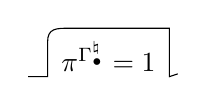
\begin{tikzpicture}[baseline=(eq.base)]
\node[inner sep=0pt,outer sep=0pt] (eq) {$\pi^{\mathbb{\Gamma}_{\bullet}^{\natural}}=1$};
\draw[line width=0.4pt]
([xshift=-12pt,yshift=-2pt]eq.south west)
-- ([xshift=-5pt,yshift=-2pt]eq.south west)
-- ([xshift=-5pt]eq.north west)
.. controls ([xshift=-5pt,yshift=5pt]eq.north west) and ([xshift=-2pt,yshift=5pt]eq.north west) .. ([xshift=3pt,yshift=5pt]eq.north west)
-- ([xshift=5pt,yshift=5pt]eq.north east)
-- ([xshift=5pt,yshift=-2pt]eq.south east)
-- ([xshift=8pt,yshift=-1pt]eq.south east);
\end{tikzpicture}}
(ceci pour \deleted{\unsure{l'ad}}
\margin{403}

\scanpage{405}
\mspage{205}
l'admissibilité.

\uline{Question liminaire} La connaissance de
$\pi$, de $\underbrace{\widehat{\mathcal T}_a^+}_{\Sigma_a}
\subset\widehat{\widehat{\mathcal T}}(\pi)$, et \unsure{d'un} ss-groupe
$\Gamma'\subset\widehat{\widehat{\mathcal T}}(\pi)$
(normalisant $\Sigma_a$, \inserted{tel que
$\Gamma'\cap\unsure{\Sigma_a|\Sigma_{\bullet}}=(1)$})
\unsure{permettrait-il} de retrouver l'\unsure{arithmatisation|arithmétisation} de $\pi$
--- et, pour commencer, de retrouver
$\mathcal N_a$ (dans lequel $\Gamma'\cdot\Sigma$ est d'indice
fini) ? \deleted{Est} Il \unsure{suffirait|suffira}, pour pouvoir
répondre par l'affirmative, de savoir
que tt \unsure{isom.} ext. $\pi\longrightarrow\pi_{g,\nu}$,
qui envoie \inserted{$\Sigma$ sur $\widehat{\mathcal T}_{g,\nu}=\Sigma_{g,\nu}$, et}
\unsure{tt|le} ss-groupe d'indice
fini $\Gamma'\cdot\Sigma$ dans $\mathcal N_a$ dans $\mathcal N_{g,\nu}$,
est compatible avec les \unsure{arithmatisations|arithmétisations}.
Or ceci revient \unsure{exactt|exactmt} :

\textcircled{g} (facultatif, quand même !)
\deleted{tout} Pour tt sous-groupe
ouvert $\mathcal N'$ de $\mathcal N_{g,\nu}$,
les éléments de $\widehat{\widehat{\mathcal T}}_{g,\nu}$
\inserted{normalisant $\widehat{\mathcal T}_{g,\nu}$ et}
qui transportent
$\mathcal N'$ dans $\mathcal N_{g,\nu}$, \unsure{sont} dans $\mathcal N_{g,\nu}$
(\unsure{a fortiori},
$\mathcal N_{g,\nu}$ serait son propre normalisateur
dans $\operatorname{Norm}_{\widehat{\widehat{\mathcal T}}_{g,\nu}}
(\widehat{\mathcal T}_{g,\nu})$.
\margin{404}

\scanpage{406}
Avec les ``points de $U$'' (définis comme \unsure{classes}
de conjugaison de \unsure{relèvts} (19)
``admissibles'' i.e. satisfaisant (20), on
fait un groupoïde, ayant comme
groupe fondamental extérieur $\pi$, et sur
lequel $\Gamma^{\unsure{\natural|\sharp}}\subset\mathcal N_a$ opère strictement
(\uline{NB} pour se reposer, on se donne
maintenant $\unsure{\Gamma^{\natural}|\Gamma}$ lui-$\overline{\mathrm m}$, pas \unsure{seulmt|seulement} un
germe --- \unsure{moralmt|moralement}, cela signifie
qu'on a une courbe définie sur une
sous-ext. finie $K$ de $\overline{\mathbb Q}/\mathbb Q$ \ldots\unsure{\}|)}.
Les pts fixes de $\Gamma$ correspondent
aux pts rat/$K$, les pts fixes sous un
ss-groupe fermé $\Gamma'$ aux pts rationnels
sur la sous-extension $K'$ de $\overline{\mathbb Q}/\mathbb Q$ asso-
ciée à $\Gamma'$ \ldots)
\margin{405}

\scanpage{407}
\mspage{206}

Soit maintenant
\figure{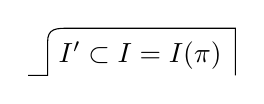
\begin{tikzpicture}[baseline=(eq.base)]
\node[inner sep=0pt,outer sep=0pt] (eq) {$I'\subset I=I(\pi)$};
\draw[line width=0.4pt]
([xshift=-11pt,yshift=-2pt]eq.south west)
-- ([xshift=-4pt,yshift=-2pt]eq.south west)
-- ([xshift=-4pt]eq.north west)
.. controls ([xshift=-4pt,yshift=5pt]eq.north west) and ([xshift=-1pt,yshift=5pt]eq.north west) .. ([xshift=4pt,yshift=5pt]eq.north west)
-- ([xshift=5pt,yshift=5pt]eq.north east)
-- ([xshift=5pt,yshift=-2pt]eq.south east);
\end{tikzpicture}}
une
partie de $I$, stable par $\Gamma$. On trouve
par "bouchage des trous en $I'$" un
groupe ext. à lacets $\pi'$, \deleted{qui} et un
hom extérieur
\[
(20)\qquad \pi^{\unsure{\natural|\sharp}}\longrightarrow\pi'
\]
D'ailleurs $\pi'$ hérite d'une arithmétisation \inserted{$a'$}
par $\pi$ -- et on aura
\[
(21)\qquad
\left\{
\begin{array}{ccc}
\mathbb{\Gamma}_a & \overset{\sim}{\longrightarrow} & \mathbb{\Gamma}_{a'} \\
\mathbb P_a & \overset{\sim}{\longrightarrow} & \mathbb P_{a'} \\
\unsure{\wr} & & \\
P & &
\end{array}
\right.
\quad\unsure{\leadsto}
\]
donc $\pi'$ est défini sur \unsure{le|la} $\overline{\mathrm m}$ $P$ que
$\mathbb{\Gamma}_a$
(i.e. en faisant des trous dans $U$ pour
trouver $U'$, on n'a pas dérangé le
corps de base alg. \unsure{clos|abs} $\overline{\mathbb Q}\ldots$). D'ailleurs
on aura un hom canonique
\[
\widehat{\mathcal T}(\pi)\longrightarrow
\widehat{\mathcal T}(\pi')
\]
induisant
\begin{samepage}
\[
(22)\qquad
\]
\diagram{\begin{tikzcd}[ampersand replacement=\&,column sep=3.2em,row sep=1.8em]
\mathcal N_a \arrow[r] \arrow[d,phantom,"\cup" description] \& \mathcal N_{a'} \arrow[d,phantom,"\cup" description] \\
\widehat{\mathcal T}_a \arrow[r,dash] \& \widehat{\mathcal T}_{a'}
\end{tikzcd}}
\end{samepage}

\margin{406}

\scanpage{408}

(induisant justement $\mathbb{\Gamma}_a\longrightarrow\mathbb{\Gamma}_{a'}$ par passage
aux quotients), et on trouve, en
composant
\[
\Gamma\;\unsure{\subset|\hookrightarrow}\;\mathcal N_a\longrightarrow\mathcal N_{a'}
\]
un hom \unsure{égalmt|également} injectif
\[
(23)\qquad\Gamma\hookrightarrow\mathcal N_{a'}
\]
qui est une \unsure{quasi-section|quasi section} de $\mathcal N_{a'}$ sur $\mathbb{\Gamma}_{a'}$,
Donc \deleted{\unsure{que|par}}\inserted{sous} réserve d'admissibilité,
on trouve sur \deleted{\illegible{1}} $\unsure{\pi'|\pi}$ une structure
de courbe algébrique potentielle, relatif
au $\overline{\mathrm m}$ $P$.

\deleted{L'admissibilité s'exprime
\unsure{peut-être par} la condition
\[
(24)\qquad {\pi'}^{\Gamma}=(1)
\]
-- et s'il le faut, on mettra ces
conditions (pour \unsure{tte|$\forall$} $I'\subset I$) dans
la définition de l'admissibilité de}

\deleted{\illegible{1} \unsure{Je}} Je suis vraiment gêné
aux entournures, faute d'avoir une
définition en forme de "admissible" --

\margin{407}

\scanpage{409}
\mspage{207}

je vais y revenir très vite --- mais
pour le moment, j'ai envie de noter que,
\deleted{du fait que $\Gamma$ \unsure{opérait} \unsure{tr.}}
\inserted{si $I'\neq\varnothing$,}
le groupe ext. $\pi'$ peut se décrire par
un \inserted{vrai} groupoïde, ayant $I'$ comme ens.
d'objets, et sur lequel $\Gamma$ opère en
sens strict (ceci est de l'algèbre pure,
indépendamment des histoires d'arithmétisation\ldots)
Le fait que $\Gamma$ opère \unsure{trivialt}
sur les $i'\in I'$ implique que pour \unsure{tt|$\forall$}
$i'\in I'$, on a un \deleted{\unsure{relèvement de}}
\unsure{hom.} canonique
\[
(24)\qquad \Gamma\longrightarrow\pi'(i')
\]
qui relève son action \unsure{extérieur|extérieure}, d'où
une \unsure{uq} classe de \inserted{$\pi'$-}conj. de relèvements
de l'action ext. de $\Gamma$ sur $\pi'$
en une vraie action de $\Gamma$ sur $\pi'$
--- on espère qu'elle satisfait ${\pi'}^{\Gamma}=1$ ---
et on a donc une application can.
\[
(25)\qquad I'\longrightarrow\mathrm{Pts}(\pi',\alpha',\Gamma)
\]

\margin{408}

\scanpage{410}

Je \uline{dis que cette application est injective}

Ceci est "évident" quand on interprète
"action ext. admissible" par "réalisable
par une vraie courbe alg.", et
"relèvements admissibles" par "réalisables
par des vrais pts rat / \unsure{$K^+$|$K$}, corps des
\unsure{fixes|invariants} de $\Gamma$". Mais on voudrait
bien sûr des raisons internes à
la donnée des $(\mathcal N_{g,\nu})$, et des \unsure{)}
propriétés de ces données ! \deleted{\unsure{Et}}

\margin{On \unsure{est ramené|va revenir} au cas Card $I'=2$\ldots}

Ce pt étant admis (en mettant
entre parenthèses les deux définitions
\unsure{éventuelles|essentielles} d'admissibilité, sur lesquelles
on va revenir plus bas) on trouve
un foncteur "bouchage de trous"
\diagram{\begin{tikzcd}[ampersand replacement=\&,column sep=large]
\begin{gathered}
\text{Courbes algébriques}\\
\text{potentielles sur }P,\ \text{\unsure{\deleted{relatives}|relatives}}\\
\text{à un ss-groupe ouvert}\\
\text{\deleted{\unsure{d'un ens}}}\\
\Gamma\text{ de }\mathbb{\Gamma}_P,\ \text{et munies d'un}\\
\text{ens }I'\text{ de pts à l'}\infty
\end{gathered}
\arrow[r]
\&
\begin{gathered}
\text{Courbes alg.}\\
\text{pot. sur }P\text{ relatives}\\
\text{à }\Gamma,\ \text{munies}\\
\text{d'une partie}\\
\text{de l'ens des}\\
\text{"Pts \unsure{ratls|invts}/}\Gamma\text{"}
\end{gathered}
\end{tikzcd}}

\margin{il faut pour ceci les restrictions
anabéliennes habituelles}

\margin{409}
